% LaTeX Article Template
\documentclass{article}
\usepackage{amssymb, amsmath, amsfonts, amsthm, latexsym, graphicx, enumitem}
\newcommand{\C}{\mathbb {C}}
\newcommand\tab[1][1cm]{\hspace*{#1}}
\newcommand\smalltab[1][0.3cm]{\hspace*{#1}}

\begin{document}

\begin{center}
\textbf{CSCI 362 Deliverable 3: SugarLabs}
\end{center}


\begin{center}

{The Chocolate L'Eclercs}\\
\vspace{0.2cm}
{Alex Skiff, Blaine Billings, Carson Barber}\\
{Chase Myers, Justin Willis}\\
\vspace{0.2cm}

\end{center}

\section{Deliverable 3: Automated Testing Framework}
\subsection{Architectural Description}
The automated testing framework has been subdivided in to following sections for ease of use:
\begin{itemize}[noitemsep,topsep=0pt]
\item[]\rotatebox[origin=c]{180}{$\Lsh$}\textbf{/TestAutomation}: Root directory for the automated testing framework
\begin{itemize}[noitemsep,topsep=0pt]
\item[]\rotatebox[origin=c]{180}{$\Lsh$}\textbf{/sugar}: Contains the cloned project files for the SugarLabs repository
\item[]\rotatebox[origin=c]{180}{$\Lsh$}\textbf{/scripts}: Contains scripts used for running a specific test case and for running all test cases
\item[]\rotatebox[origin=c]{180}{$\Lsh$}\textbf{/testCases}: Contains test case input
\item[]\rotatebox[origin=c]{180}{$\Lsh$}\textbf{/testCaseExecutables}: Contains the test cases written in python
\item[]\rotatebox[origin=c]{180}{$\Lsh$}\textbf{/temp}: Contains the output.log file where all testing output is piped
\item[]\rotatebox[origin=c]{180}{$\Lsh$}\textbf{/docs}: Contains the README.txt file for the automated testing framework
\item[]\rotatebox[origin=c]{180}{$\Lsh$}\textbf{/reports}: Contains all of the reports associated with the automated testing framework
\end{itemize}
\end{itemize}
\subsection{Documentation}
Each of the test cases have been written and saved to the /TestAutomation/testCaseExecutables folder, with their input files being located in /TestAutomation/testCases as described above. In each of these testCase input files is outlined a brief description of the test case and how one may go about modifying it for their own purposes. An example of such is provided in Figure \ref{Figure3}
\begin{figure}
\centering
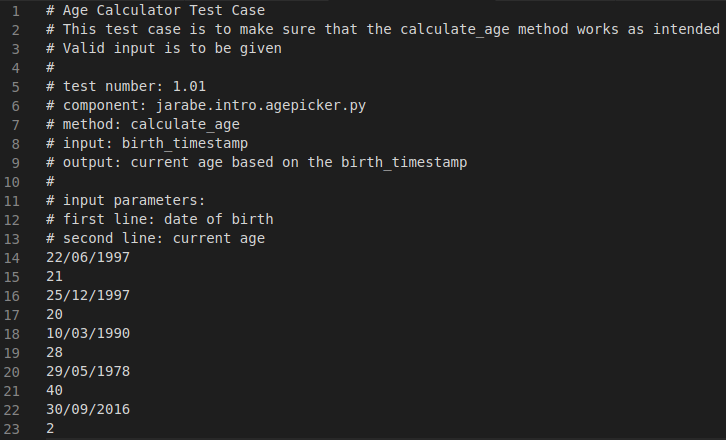
\includegraphics[scale=0.4]{../imgs/Figure3.png}
\caption{Example documentation for testCase input files, allowing users to be able to understand how to modify them as necessary.}
\label{Figure3}
\end{figure}
\subsection{Test Case Sepcifications}
For the first step in the implementation of our automate testing framework we wrote and exectuted five primary test cases. These are specified below.
\begin{itemize}[noitemsep]
\item age\_calculator
\begin{itemize}[noitemsep,topsep=0pt]
\item \textbf{Test ID}: 1.01
\item \textbf{Test Requirement}: Correlated age input is properly recognized by the system as correct input and subsequently processed.
\item \textbf{Test Component}: jarabe.intro.agepicker
\item \textbf{Test Method}: calculate\_age
\item \textbf{Test Input}: Input is provided in the form of two-line input, the first being the birthdate of the user and the second the correct age of said user. Input: (22/06/1997, 21), (25/12/1997, 20), (10/03/1990, 28), (29/05/1978, 40), (30/09/2016, 2)
\item \textbf{Expected Output}: Output is expected to return True for each of the input test cases, as the calculated age and input age will match. Expected Output: True, True, True, True, True
\end{itemize}
\item age\_calculator\_invalid
\begin{itemize}[noitemsep,topsep=0pt]
\item \textbf{Test ID}: 1.02
\item \textbf{Test Requirement}: Noncorrelated age input is properly recognized by the system as incorrect input.
\item \textbf{Test Component}: jarabe.intro.agepicker
\item \textbf{Test Method}: calculate\_age
\item \textbf{Test Input}: Input is provided in the form of two-line input, the first being the birthdate of the user and the second the correct age of said user. Input: (22/06/1997, 22), (25/12/1997, 21), (10/03/1990, 29), (29/05/1978, 41), (30/09/2016, 3)
\item \textbf{Expected Output}: Output is expected to return False for each of the input test cases, as the calculated age and input age will match. Expected Output: False, False, False, False, False
\end{itemize}
\item buddy\_nickname
\begin{itemize}[noitemsep,topsep=0pt]
\item \textbf{Test ID}: 2.01
\item \textbf{Test Requirement}: A user must be able to set and be returned the nickname of their account's "buddy"
\item \textbf{Test Component}: jarabe.model.buddy
\item \textbf{Test Method}: set\_nick, get\_nick
\item \textbf{Test Input}: Input is provided in the form of a string, representing the buddy nickname. Input: bigboidan
\item \textbf{Expected Output}: Output is expected to return the input string for each of the input test cases, as the set method should properly set the nickname, and the get method should properly return the nickname. Expected Output: bigboidan
\end{itemize}
\item buddy\_key
\begin{itemize}[noitemsep,topsep=0pt]
\item \textbf{Test ID}: 2.02
\item \textbf{Test Requirement}: A user must be able to set and be returned the key of their account's "buddy"
\item \textbf{Test Component}: jarabe.model.buddy
\item \textbf{Test Method}: set\_key, get\_key
\item \textbf{Test Input}: Input is provided in the form of a two eight-letter codes joined by an underscore, representing the buddy key. Input: DEADBEEF\_DEADCODE
\item \textbf{Expected Output}: Output is expected to return the input key for each of the input test cases, as the set method should properly set the key, and the get method should properly return the key. Expected Output: DEADBEEF\_DEADCODE
\end{itemize}
\item buddy\_color
\begin{itemize}[noitemsep,topsep=0pt]
\item \textbf{Test ID}: 2.03
\item \textbf{Test Requirement}: A user must be able to set and be returned the color of their account's "buddy"
\item \textbf{Test Component}: jarabe.model.buddy
\item \textbf{Test Method}: set\_color, get\_color
\item \textbf{Test Input}: Input is provided in the form of a six-digit hex number, representing the buddy color. Input: FF00FF
\item \textbf{Expected Output}: Output is expected to return the input number for each of the input test cases, as the set method should properly set the color, and the get method should properly return the color. Expected Output: FF00FF
\end{itemize}
\end{itemize}

\end{document}